%% ============================================================
%%  CHAPTER 5 — SIGNAL PROCESSING PIPELINE
%% ============================================================
\chapter{Signal Processing Pipeline}
\label{ch:signal_processing}

This chapter presents the complete signal processing pipeline
applied to the raw \acrshort{eeg} recordings before feature
extraction. Section~\ref{sec:sp_overview} provides a pipeline
overview. Section~\ref{sec:sp_loading} describes \acrshort{edf}
file loading and channel configuration. Section~\ref{sec:sp_notch}
derives the notch filter used to suppress power-line interference.
Section~\ref{sec:sp_bandpass} derives the bandpass filter used
to isolate the frequency range of interest. Section~\ref{sec:sp_car}
describes Common Average Reference spatial normalisation.
Section~\ref{sec:sp_epoch} covers epoch extraction and overlap
strategy. Section~\ref{sec:sp_reject} describes amplitude-based
artifact rejection. Section~\ref{sec:sp_gate} presents the
activity-gated epoch selection mechanism — the key innovation
of this pipeline. Section~\ref{sec:sp_norm} describes per-recording
Z-score normalisation. Section~\ref{sec:sp_summary} summarises
the chapter.

%% ----------------------------------------------------------
\section{Pipeline Overview}
\label{sec:sp_overview}
%% ----------------------------------------------------------

The signal processing pipeline transforms raw multichannel
\acrshort{eeg} recordings into a set of clean, labelled, 
activity-gated epoch arrays suitable for feature extraction.
Figure~\ref{fig:sp_pipeline} illustrates the complete sequence
of processing stages applied to each \acrshort{edf} file.

\begin{figure}[htbp]
\centering
\begin{tikzpicture}[
    node distance=0.5cm,
    box/.style={rectangle, rounded corners=3pt, draw=black,
                fill=blue!10, minimum width=5.5cm,
                minimum height=0.75cm, align=center,
                font=\small},
    decision/.style={diamond, draw=black, fill=yellow!20,
                     minimum width=3cm, minimum height=0.8cm,
                     align=center, font=\small},
    arrow/.style={-{Stealth[length=5pt]}, thick},
    note/.style={font=\scriptsize\itshape, text=gray,
                 align=left}
]

\node[box, fill=green!15]  (load)  {1.\ Load EDF File};
\node[box, below=of load]  (notch) {2.\ Notch Filter (50/60\,Hz)};
\node[box, below=of notch] (bp)    {3.\ Bandpass Filter (1--45\,Hz)};
\node[box, below=of bp]    (car)   {4.\ Common Average Reference (CAR)};
\node[box, below=of car]   (epoch) {5.\ Epoch Extraction (2.0\,s, 50\% overlap)};
\node[decision, below=of epoch] (reject)
    {Amplitude $> \pm$150\,\si{\micro\volt}?};
\node[box, right=2cm of reject, fill=red!15] (drop1)
    {Discard epoch};
\node[decision, below=of reject] (gate)
    {RMS energy $<$ threshold?};
\node[box, right=2cm of gate, fill=red!15] (drop2)
    {Discard epoch\\(rest window)};
\node[box, below=of gate]  (norm)  {6.\ Per-Recording Z-Score Normalisation};
\node[box, below=of norm, fill=orange!20]  (feat)
    {$\rightarrow$ Feature Extraction (Chapter~6)};

\draw[arrow] (load)  -- (notch);
\draw[arrow] (notch) -- (bp);
\draw[arrow] (bp)    -- (car);
\draw[arrow] (car)   -- (epoch);
\draw[arrow] (epoch) -- (reject);
\draw[arrow] (reject) -- node[right,font=\scriptsize]{Yes} (drop1);
\draw[arrow] (reject) -- node[right,font=\scriptsize]{No}  (gate);
\draw[arrow] (gate)   -- node[right,font=\scriptsize]{Yes} (drop2);
\draw[arrow] (gate)   -- node[right,font=\scriptsize]{No}  (norm);
\draw[arrow] (norm)  -- (feat);

%% Side annotations
\node[note, right=0.3cm of load]
    {loader.py: pyEDFlib, 19 ch, 200\,Hz};
\node[note, right=0.3cm of notch]
    {2nd-order IIR, zero-phase};
\node[note, right=0.3cm of bp]
    {4th-order Butterworth, zero-phase};
\node[note, right=0.3cm of car]
    {$x_{i}^{\text{CAR}} = x_i - \bar{x}$};
\node[note, right=0.3cm of epoch]
    {400 samples/epoch, 200-sample step};
\node[note, right=0.3cm of norm]
    {$z = (x - \mu)/\sigma$ per recording};

\end{tikzpicture}
\caption{Complete signal processing pipeline applied to each
EDF recording file. Epochs failing the amplitude threshold are
discarded as corrupted. Epochs below the RMS activity threshold
are discarded as rest windows. Only active, clean epochs proceed
to feature extraction.}
\label{fig:sp_pipeline}
\end{figure}

All processing stages are implemented in \code{preprocessing.py}
using \textit{NumPy}~\cite{harris2020numpy} and
\textit{SciPy}~\cite{virtanen2020scipy}. The pipeline is
applied identically during both offline training and real-time
inference, ensuring train--inference consistency — a critical
requirement for reliable deployment.

%% ----------------------------------------------------------
\section{EDF File Loading and Channel Configuration}
\label{sec:sp_loading}
%% ----------------------------------------------------------

Raw \acrshort{eeg} recordings are stored in European Data Format
(\acrshort{edf}), a standard format for multichannel biological
signals~\cite{kemp1992edf}. Each \acrshort{edf} file is loaded
using the \textit{pyEDFlib} library, which reads the file header
to extract the channel labels, sampling frequency, and signal
duration, then reads the raw sample arrays for all channels.

The loader performs the following steps for each \acrshort{edf}
file:

\begin{enumerate}[leftmargin=*]
    \item \textbf{Header parsing:} Extract channel labels,
    sampling frequency (\SI{200}{\hertz}), and total number
    of samples.
    \item \textbf{Channel ordering:} Map the channel labels
    to the standard 19-channel 10--20 order:
    \{Fp1, Fp2, F7, F3, Fz, F4, F8, T3, C3, Cz, C4, T4,
    T5, P3, Pz, P4, T6, O1, O2\}.
    \item \textbf{Signal array assembly:} Load all 19 channel
    arrays and stack them into a matrix $\mathbf{X} \in
    \mathbb{R}^{19 \times N}$, where $N$ is the total number
    of samples in the recording.
    \item \textbf{Initial crop:} Remove the first and last
    \SI{1}{\second} of each recording to discard the
    transient period during which the subject is settling
    into position and any end-of-recording artifacts.
\end{enumerate}

The resulting signal matrix $\mathbf{X}$ has dimensions
$19 \times N_{\text{cropped}}$, where each row corresponds
to one electrode channel and each column to one time sample
at \SI{200}{\hertz}.

%% ----------------------------------------------------------
\section{Notch Filter}
\label{sec:sp_notch}
%% ----------------------------------------------------------

\subsection{Purpose}

Power-line interference at 50\,Hz (or 60\,Hz in regions using
the North American standard) introduces a strong narrowband
sinusoidal artifact into \acrshort{eeg} recordings. This
interference arises from electromagnetic induction from nearby
power cables, lighting fixtures, and electronic equipment.
Although the artifact is narrowband, its amplitude can exceed
that of the \acrshort{eeg} signals of interest, severely
distorting spectral features computed in the affected frequency
range. A notch filter is applied to attenuate this interference
while leaving the rest of the spectrum intact.

\subsection{Filter Design}

A 2nd-order Infinite Impulse Response (IIR) notch filter
is implemented using the bilinear transform of an ideal
continuous-time notch filter. The transfer function of the
continuous-time prototype is:

\begin{equation}
H_{\text{notch}}(s) = \frac{s^2 + \omega_0^2}
{s^2 + \frac{\omega_0}{Q}\,s + \omega_0^2}
\label{eq:notch_ct}
\end{equation}

\noindent where $\omega_0 = 2\pi f_0$ is the notch frequency
in radians per second ($f_0 = 50$\,Hz) and $Q$ is the quality
factor controlling the notch bandwidth. A quality factor of
$Q = 30$ was selected, yielding a $-3$\,dB bandwidth of
approximately $f_0/Q \approx 1.67$\,Hz, which is narrow enough
to avoid attenuating the adjacent spectrum while being wide
enough to suppress the power-line fundamental and its minor
frequency drift.

The discrete-time filter coefficients are computed using
\code{scipy.signal.iirnotch}:

\begin{lstlisting}[language=Python,
    caption={Notch filter implementation.},
    label={lst:notch}]
from scipy.signal import iirnotch, filtfilt

def apply_notch(signal, fs=200, f0=50.0, Q=30.0):
    """
    Apply zero-phase notch filter to suppress power-line
    interference at f0 Hz.
    signal : ndarray, shape (n_channels, n_samples)
    fs     : sampling frequency in Hz
    f0     : notch frequency in Hz
    Q      : quality factor (higher = narrower notch)
    """
    b, a = iirnotch(w0=f0, Q=Q, fs=fs)
    return filtfilt(b, a, signal, axis=1)
\end{lstlisting}

\subsection{Zero-Phase Filtering}

The filter is applied using \code{scipy.signal.filtfilt}, which
implements zero-phase filtering by processing the signal in
both forward and reverse directions. Forward-only filtering
introduces a frequency-dependent phase delay, causing the
temporal position of signal peaks to shift after filtering
— a critical distortion for blink peak timing features.
Zero-phase filtering eliminates this distortion entirely,
preserving the precise timing of artifact events at the cost
of slightly increased transient effects at the signal
boundaries (mitigated by the initial crop described in
Section~\ref{sec:sp_loading}).

The effective transfer function of the zero-phase filter is:

\begin{equation}
H_{\text{zero-phase}}(e^{j\omega}) =
\left|H(e^{j\omega})\right|^2
\label{eq:zerophase}
\end{equation}

\noindent which is purely real (zero phase) and has a
magnitude response equal to the squared magnitude of the
one-pass filter.

%% ----------------------------------------------------------
\section{Bandpass Filter}
\label{sec:sp_bandpass}
%% ----------------------------------------------------------

\subsection{Purpose and Cutoff Selection}

A bandpass filter is applied after the notch filter to isolate
the frequency range containing the signals of interest while
suppressing low-frequency drift and high-frequency noise.

The lower cutoff frequency was set to $f_L = 1$\,Hz to remove
slow DC drift and baseline wander (electrode polarisation
potentials, galvanic skin response) while preserving the slow
components of the blink waveform (which has a rise time of
approximately 150\,ms, corresponding to a fundamental frequency
of $\sim$3\,Hz). A lower cutoff of 0.5\,Hz (commonly used in
motor imagery \acrshort{bci}) would admit more drift but was
found to increase baseline instability in long recordings.

The upper cutoff frequency was set to $f_H = 45$\,Hz. This
choice reflects a balance between two competing requirements:
(1) preserving the high-frequency \acrshort{emg} components
of jaw artifact signals (bruxism and clinch), which contain
significant power up to 80\,Hz; and (2) suppressing broadband
high-frequency noise and the aliased power-line harmonic at
$f_s/2 = 100$\,Hz. A cutoff of 45\,Hz was found empirically
to retain the most discriminative jaw \acrshort{emg} energy
while limiting noise amplification.

\subsection{Filter Design}

A 4th-order Butterworth bandpass filter is used. The Butterworth
design was chosen for its maximally flat passband response —
no ripple in the passband — which avoids distorting the
amplitude of spectral features estimated in the passband.

The continuous-time Butterworth lowpass prototype of order $N$
has the transfer function:

\begin{equation}
\left|H_{\text{LP}}(j\Omega)\right|^2 =
\frac{1}{1 + \left(\Omega/\Omega_c\right)^{2N}}
\label{eq:butterworth}
\end{equation}

\noindent where $\Omega_c$ is the $-3$\,dB cutoff frequency
and $N = 4$ is the filter order. The bandpass version is
obtained by applying the standard lowpass-to-bandpass
frequency transformation. The resulting filter has order $2N
= 8$ poles in the $s$-plane, which after bilinear
transformation yields an 8th-order discrete IIR filter.

\begin{lstlisting}[language=Python,
    caption={Bandpass filter implementation.},
    label={lst:bandpass}]
from scipy.signal import butter, filtfilt

def apply_bandpass(signal, fs=200,
                   f_low=1.0, f_high=45.0, order=4):
    """
    Apply zero-phase Butterworth bandpass filter.
    signal  : ndarray, shape (n_channels, n_samples)
    fs      : sampling frequency in Hz
    f_low   : lower cutoff frequency in Hz
    f_high  : upper cutoff frequency in Hz
    order   : filter order (default 4)
    """
    nyq = fs / 2.0
    low  = f_low  / nyq
    high = f_high / nyq
    b, a = butter(order, [low, high], btype='band')
    return filtfilt(b, a, signal, axis=1)
\end{lstlisting}

\subsection{Combined Filter Response}

Figure~\ref{fig:filter_response} shows the combined magnitude
response of the notch and bandpass filters applied in sequence.

\begin{figure}[htbp]
\centering
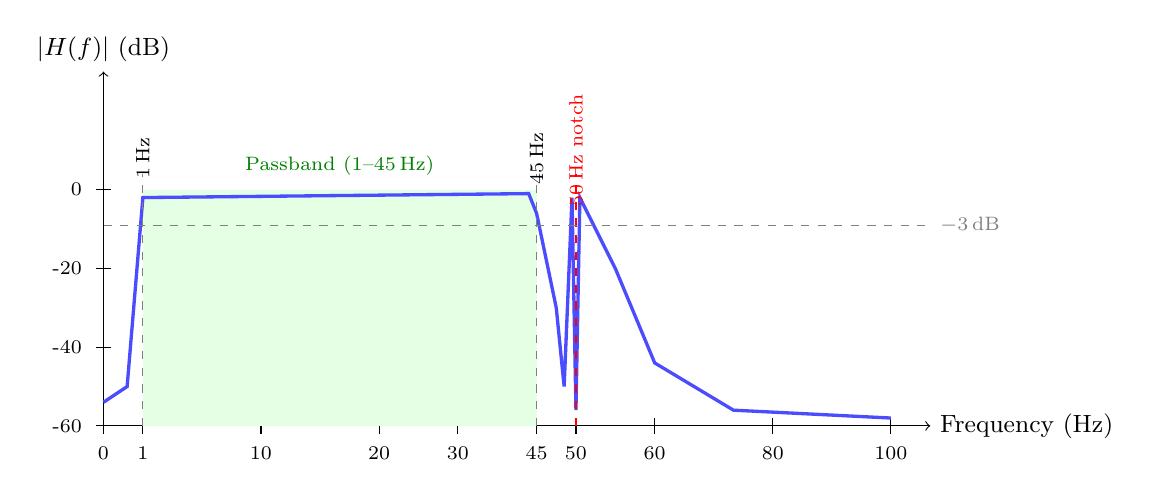
\begin{tikzpicture}[scale=1.0]
    % Axes
    \draw[->] (0,0) -- (10.5,0)
        node[right]{\small Frequency (Hz)};
    \draw[->] (0,0) -- (0,4.5)
        node[above]{\small $|H(f)|$ (dB)};

    % Y-axis ticks
    \foreach \y/\label in {0/-60, 1/-40, 2/-20, 3/0}{
        \draw (-0.1,\y) -- (0.1,\y);
        \node[left, font=\scriptsize] at (-0.15,\y) {\label};
    }

    % X-axis ticks (0,1,5,10,20,30,45,50,60,80,100Hz)
    \foreach \x/\label in {
        0/0, 0.5/1, 2.0/10, 3.5/20, 4.5/30,
        5.5/45, 6.0/50, 7.0/60, 8.5/80, 10/100}{
        \draw (\x,-0.1) -- (\x,0.1);
        \node[below, font=\scriptsize] at (\x,-0.15) {\label};
    }

    % Passband region shading
    \fill[green!10] (0.5,0) rectangle (5.5,3);

    % Filter response curve
    \draw[blue!70, very thick]
        (0.0, 0.3) -- (0.3, 0.5) -- (0.5, 2.9)
        -- (5.4, 2.95) -- (5.5, 2.7)
        -- (5.75, 1.5) -- (5.85, 0.5)
        -- (5.95, 2.9) -- (6.0, 0.2)   %% notch at 50 Hz
        -- (6.05, 2.9) -- (6.5, 2.0)
        -- (7.0, 0.8) -- (8.0, 0.2) -- (10.0, 0.1);

    % Annotations
    \draw[dashed, gray] (0.5,0) -- (0.5,3.2);
    \node[font=\scriptsize, rotate=90] at (0.5,3.4) {1\,Hz};
    \draw[dashed, gray] (5.5,0) -- (5.5,3.2);
    \node[font=\scriptsize, rotate=90] at (5.5,3.4) {45\,Hz};
    \draw[dashed, red] (6.0,0) -- (6.0,3.2);
    \node[red, font=\scriptsize, rotate=90] at (6.0,3.5)
        {50\,Hz notch};

    % Passband label
    \node[font=\scriptsize, green!50!black] at (3.0, 3.3)
        {Passband (1--45\,Hz)};

    % -3dB line
    \draw[dashed, gray, thin] (0, 2.55) -- (10.5, 2.55);
    \node[right, font=\scriptsize, gray] at (10.5, 2.55)
        {$-$3\,dB};

\end{tikzpicture}
\caption{Combined magnitude response of the notch filter
(50\,Hz) and 4th-order Butterworth bandpass filter
(1--45\,Hz). The passband (green region) passes the
blink and jaw EMG artifact signals. The notch attenuates
power-line interference. All filtering is applied
zero-phase to preserve signal timing.}
\label{fig:filter_response}
\end{figure}

%% ----------------------------------------------------------
\section{Common Average Reference}
\label{sec:sp_car}
%% ----------------------------------------------------------

\subsection{Purpose}

After bandpass filtering, a Common Average Reference
(\acrshort{car}) spatial filter is applied to the multichannel
\acrshort{eeg}. The \acrshort{car} removes spatial
common-mode noise — signals that appear with approximately
equal amplitude across all electrodes simultaneously — which
arises from electromagnetic interference, movement of the
reference electrode, and cardiac pulse artifacts.

\subsection{Mathematical Formulation}

For a signal matrix $\mathbf{X} \in \mathbb{R}^{C \times T}$,
where $C = 19$ is the number of channels and $T$ is the number
of time samples, the \acrshort{car} is defined as:

\begin{equation}
x_i^{\text{CAR}}(t) = x_i(t) - \frac{1}{C}
\sum_{k=1}^{C} x_k(t)
\quad \forall\, i \in \{1, \ldots, C\},\;
\forall\, t \in \{1, \ldots, T\}
\label{eq:car}
\end{equation}

\noindent In matrix form:

\begin{equation}
\mathbf{X}^{\text{CAR}} = \left(\mathbf{I}_C -
\frac{1}{C}\mathbf{1}_C\mathbf{1}_C^\top\right)\mathbf{X}
= \mathbf{H}\,\mathbf{X}
\label{eq:car_matrix}
\end{equation}

\noindent where $\mathbf{I}_C$ is the $C \times C$ identity
matrix, $\mathbf{1}_C$ is the $C$-dimensional all-ones vector,
and $\mathbf{H}$ is the \acrshort{car} centering matrix.

\subsection{Effect on Artifact Signals}

The \acrshort{car} is particularly beneficial for the
artifact-based \acrshort{bci} paradigm because the voluntary
artifacts (blinks, bruxism) are spatially localised to specific
electrode groups (frontal and temporal), while common-mode
interference is spatially uniform. Subtracting the spatial
mean enhances the relative amplitude of the localised artifact
signals at Fp1/Fp2 and T3/T4 compared to the global background.

\begin{lstlisting}[language=Python,
    caption={Common Average Reference implementation.},
    label={lst:car}]
import numpy as np

def apply_car(signal):
    """
    Apply Common Average Reference spatial filter.
    signal : ndarray, shape (n_channels, n_samples)
    Returns: CAR-referenced signal, same shape
    """
    return signal - signal.mean(axis=0, keepdims=True)
\end{lstlisting}

Note that \code{signal.mean(axis=0)} computes the mean across
channels at each time point (the spatial mean), which is then
subtracted from each channel — equivalent to Equation
\eqref{eq:car}.

%% ----------------------------------------------------------
\section{Epoch Extraction}
\label{sec:sp_epoch}
%% ----------------------------------------------------------

\subsection{Windowing Strategy}

After \acrshort{car} referencing, the continuous preprocessed
signal is divided into fixed-length overlapping windows
(epochs). The epoch parameters were selected as follows:

\begin{itemize}[leftmargin=*]
    \item \textbf{Epoch duration:} $T_{\text{epoch}} =
    2.0$\,s ($= 400$ samples at \SI{200}{\hertz}). This
    duration is sufficient to capture a complete double blink
    (two peaks separated by up to 600\,ms) and a complete
    triple blink (three peaks spanning up to 1{,}200\,ms),
    while remaining short enough that the signal statistics
    are approximately stationary within each epoch.

    \item \textbf{Epoch step (overlap):} $T_{\text{step}} =
    0.5$\,s ($= 100$ samples), corresponding to 75\% overlap
    between adjacent epochs ($= 1 - 100/400$). This high
    overlap ensures that gesture events near epoch boundaries
    are captured in at least one epoch where they appear
    approximately centred.
\end{itemize}

\subsection{Mathematical Formulation}

For a preprocessed signal matrix $\mathbf{X}^{\text{CAR}}
\in \mathbb{R}^{C \times N}$, the $k$-th epoch is defined as:

\begin{equation}
\mathbf{E}_k = \mathbf{X}^{\text{CAR}}_{:,\;
k \cdot S \;:\; k \cdot S + W}
\quad k = 0, 1, 2, \ldots, K-1
\label{eq:epoch}
\end{equation}

\noindent where $W = 400$ samples is the epoch width,
$S = 100$ samples is the step size, and
$K = \lfloor (N - W) / S \rfloor + 1$ is the total
number of epochs extracted from the recording. Each epoch
$\mathbf{E}_k \in \mathbb{R}^{C \times W}$ is assigned the
class label of the \acrshort{edf} file from which it was
extracted (e.g., all epochs from \code{BLINK02.edf} are
labelled \code{double\_blink}).

\subsection{Overlap and Data Leakage Implications}

The 75\% overlap between adjacent epochs means that
consecutive epochs share 300 out of 400 samples. If these
overlapping epochs are split randomly between training and
test sets, an epoch in the test set will share 300 samples
with an epoch in the training set — constituting a severe
form of data leakage that artificially inflates test accuracy.
This issue and its resolution are discussed in detail in
Chapter~7. The overlap parameter was ultimately retained at
75\% because it improves the robustness of real-time inference
(more frequent predictions per second) and the activity gate
(finer temporal resolution for distinguishing active from rest
windows), with the data leakage addressed at the evaluation
methodology level rather than by reducing overlap.

%% ----------------------------------------------------------
\section{Amplitude-Based Artifact Rejection}
\label{sec:sp_reject}
%% ----------------------------------------------------------

Despite the preprocessing pipeline, occasional epochs contain
extreme-amplitude transients caused by electrode pop artifacts
(sudden electrode contact loss), movement artifacts, or
electrostatic discharge. These epochs, if included in training,
can distort the classifier's learned decision boundaries by
providing unrealistically large feature values.

An amplitude-based rejection criterion is applied: any epoch
in which the peak-to-peak amplitude of any channel exceeds
$\pm 150$\,\si{\micro\volt} is discarded before feature
extraction.

\begin{equation}
\text{Reject epoch } \mathbf{E}_k \text{ if: }
\max_{i,t}\left|E_k(i,t)\right| > 150\;\si{\micro\volt}
\label{eq:amplitude_reject}
\end{equation}

The threshold of 150\,\si{\micro\volt} was chosen to be above
the expected amplitude of voluntary artifact signals
(blink peaks: 50--200\,\si{\micro\volt}; bruxism/clinch:
30--100\,\si{\micro\volt} after bandpass filtering) while
below the amplitude of genuine electrode pop artifacts
(typically 300--1{,}000\,\si{\micro\volt}). In practice,
fewer than 2\% of epochs were rejected by this criterion
across both sessions.

%% ----------------------------------------------------------
\section{Activity-Gated Epoch Selection}
\label{sec:sp_gate}
%% ----------------------------------------------------------

Activity-gated epoch selection is the most significant
innovation in the preprocessing pipeline. This section provides
a complete description of the motivation, design, and
implementation of the activity gate.

\subsection{The Resting Window Problem}

Every \acrshort{edf} recording in the dataset is a single
continuous session in which the subject alternates between
performing the target gesture and resting between gestures.
For example, in \code{BLINK02.edf}, the subject performs a
double blink, rests for 3--4 seconds, performs another double
blink, and so on. The entire recording is labelled
\code{double\_blink} because that is the artifact class being
recorded.

When epochs are extracted using a sliding window without any
activity criterion, approximately 48\% of the resulting epochs
correspond to rest windows — periods during which the subject
is sitting quietly between gestures. These rest epochs contain
only background \acrshort{eeg} and are indistinguishable from
rest epochs in any other class recording. Specifically:

\begin{itemize}[leftmargin=*]
    \item A rest epoch from \code{BLINK02.edf} is labelled
    \code{double\_blink} but looks identical to background EEG.
    \item A rest epoch from \code{BLINK03.edf} is labelled
    \code{triple\_blink} but looks identical to the same
    background EEG.
    \item A rest epoch from \code{clinch.edf} is labelled
    \code{clinch} but again looks identical.
\end{itemize}

The classifier is presented with multiple instances of
identical-looking background \acrshort{eeg} carrying different
and contradictory class labels. This is an irreducible
labelling error that cannot be resolved by any classifier, and
it manifests as systematic confusion between classes in the
learned decision boundary.

\subsection{Activity Gate Design}

The activity gate addresses the resting window problem by
computing a measure of signal energy for each epoch and
discarding epochs whose energy falls below a threshold. The
gate is designed to pass only epochs that contain active
gesture signals, which have significantly higher energy than
background \acrshort{eeg}.

The energy measure is computed as the maximum \acrshort{rms}
amplitude across the two physiologically most informative
channel groups:

\begin{equation}
A_k = \max\!\left(
\text{RMS}\!\left(\mathbf{E}_k[\text{Fp1, Fp2}, :]\right),\;
\text{RMS}\!\left(\mathbf{E}_k[\text{T3, T4}, :]\right)
\right)
\label{eq:activity}
\end{equation}

\noindent where $\text{RMS}(\mathbf{v}) =
\sqrt{\frac{1}{|\mathbf{v}|}\sum_i v_i^2}$ is the Root Mean
Square of a vector, and $\mathbf{E}_k[\text{Fp1, Fp2}, :]$
denotes the rows of epoch $\mathbf{E}_k$ corresponding to
channels Fp1 and Fp2.

The epoch is retained if and only if:

\begin{equation}
A_k \geq \theta_{\text{gate}}
\label{eq:gate_criterion}
\end{equation}

\noindent where $\theta_{\text{gate}} = 20\;\si{\micro\volt}$
is the activity threshold.

\subsection{Threshold Calibration}

The threshold value $\theta_{\text{gate}} = 20\;\si{\micro\volt}$
was determined empirically by analysing the RMS amplitude
distribution of epochs from both rest windows and active
gesture windows:

\begin{itemize}[leftmargin=*]
    \item \textbf{Rest windows:} RMS amplitude at Fp1/Fp2 and
    T3/T4 during quiet rest is typically
    7--13\,\si{\micro\volt} (dominated by background
    \acrshort{eeg} alpha and beta oscillations).
    \item \textbf{Active blink epochs:} RMS amplitude at
    Fp1/Fp2 during a blink is typically
    30--150\,\si{\micro\volt}.
    \item \textbf{Active jaw epochs:} RMS amplitude at T3/T4
    during clinch/bruxism is typically
    25--100\,\si{\micro\volt}.
\end{itemize}

A threshold of 20\,\si{\micro\volt} lies comfortably in the
gap between the rest distribution (7--13\,\si{\micro\volt})
and the active gesture distribution (25--150\,\si{\micro\volt}),
providing robust separation with minimal misclassification
in either direction.

\begin{lstlisting}[language=Python,
    caption={Activity gate implementation.},
    label={lst:gate}]
import numpy as np

ACTIVITY_THRESHOLD = 20.0  # microvolts

def activity_gate(epoch, ch_names,
                  threshold=ACTIVITY_THRESHOLD):
    """
    Returns True if epoch contains active gesture signal.
    epoch    : ndarray, shape (n_channels, n_samples)
    ch_names : list of channel name strings
    threshold: RMS threshold in microvolts
    """
    fp_idx = [ch_names.index(c)
              for c in ['Fp1','Fp2'] if c in ch_names]
    t_idx  = [ch_names.index(c)
              for c in ['T3','T4'] if c in ch_names]

    rms_fp = np.sqrt(np.mean(epoch[fp_idx, :]**2))
    rms_t  = np.sqrt(np.mean(epoch[t_idx,  :]**2))

    activity = max(rms_fp, rms_t)
    return activity >= threshold
\end{lstlisting}

\subsection{Impact of Activity Gating}

The activity gate retains approximately 48\% of all extracted
epochs across all classes (see Table~\ref{tab:dataset_stats}
in Chapter~4). The consistent retention rate across classes
indicates that the gate is responding to gesture activity rather
than any class-specific property of the background
\acrshort{eeg}.

The quantitative impact on classification accuracy was
measured by comparing model performance with and without the
activity gate on the same dataset:

\begin{equation}
\Delta\text{Accuracy}_{\text{gate}} =
85.2\% - 82.1\% = +3.1\%
\label{eq:gate_improvement}
\end{equation}

This 3.1\% improvement is entirely attributable to the removal
of conflicting rest-window labels from the training set. The
improvement would be expected to grow further as more sessions
are added (more data, more rest windows to remove) and diminish
as gesture duration per recording increases relative to rest
duration.

%% ----------------------------------------------------------
\section{Per-Recording Z-Score Normalisation}
\label{sec:sp_norm}
%% ----------------------------------------------------------

\subsection{Motivation}

Absolute amplitude features — such as \acrshort{rms} and
\acrshort{ptp} computed directly from the raw signal values
— vary substantially across recording sessions due to
differences in electrode impedance, scalp moisture, amplifier
gain settings, and DC offset. A feature value of
50\,\si{\micro\volt} in Session1 may correspond to a
completely different gesture energy than the same value in
Session2, because the absolute scaling of the signal differs
between sessions.

If features are computed from unnormalised signals, the
classifier learns to exploit these inter-session amplitude
differences rather than the gesture-specific morphological
patterns. The result is a model that performs well within
a session but degrades significantly when evaluated on a
different session.

\subsection{Normalisation Procedure}

Per-recording Z-score normalisation is applied to each
\acrshort{edf} recording independently before epoch extraction.
For each channel $i$, the normalised signal is:

\begin{equation}
\tilde{x}_i(t) = \frac{x_i(t) - \mu_i}{\sigma_i + \epsilon}
\label{eq:zscore}
\end{equation}

\noindent where $\mu_i = \frac{1}{T}\sum_{t=1}^{T} x_i(t)$
is the channel mean, $\sigma_i = \sqrt{\frac{1}{T}
\sum_{t=1}^{T}(x_i(t) - \mu_i)^2}$ is the channel standard
deviation, both computed over the entire recording duration $T$,
and $\epsilon = 10^{-8}$ is a small constant added to prevent
division by zero in flat channels.

\begin{lstlisting}[language=Python,
    caption={Per-recording Z-score normalisation.},
    label={lst:zscore}]
import numpy as np

def zscore_recording(signal, eps=1e-8):
    """
    Apply per-channel Z-score normalisation to an
    entire recording before epoch extraction.
    signal : ndarray, shape (n_channels, n_samples)
    Returns: normalised signal, same shape
    """
    mu    = signal.mean(axis=1, keepdims=True)
    sigma = signal.std(axis=1,  keepdims=True)
    return (signal - mu) / (sigma + eps)
\end{lstlisting}

\subsection{Effect on Cross-Session Generalisation}

After Z-score normalisation, all channels have zero mean and
unit standard deviation within each recording. The absolute
amplitude information is discarded, and only the relative
temporal structure of the signal is preserved. Complementary
amplitude-invariant features — relative band power and Hjorth
parameters (Chapter~6) — are extracted from the normalised
signal, further reducing sensitivity to inter-session
amplitude variability.

%% ----------------------------------------------------------
\section{Pipeline Parameter Summary}
\label{sec:sp_params}
%% ----------------------------------------------------------

Table~\ref{tab:pipeline_params} summarises all signal
processing parameters with their values and justifications.

\begin{table}[htbp]
\centering
\caption{Signal processing pipeline parameter summary.}
\label{tab:pipeline_params}
\renewcommand{\arraystretch}{1.3}
\begin{tabular}{p{3.0cm} p{2.0cm} p{4.5cm}}
\toprule
\textbf{Parameter} & \textbf{Value} & \textbf{Justification} \\
\midrule
Notch frequency    & 50\,Hz     & Power-line suppression \\
Notch Q factor     & 30         & Narrow notch ($\sim$1.7\,Hz BW) \\
Bandpass low       & 1\,Hz      & Remove DC drift, keep blink shape \\
Bandpass high      & 45\,Hz     & Include jaw EMG, limit noise \\
Bandpass order     & 4          & Flat passband, adequate roll-off \\
Filter type        & Zero-phase & Preserve signal timing \\
Epoch duration     & 2.0\,s     & Capture full triple blink \\
Epoch step         & 0.5\,s     & 75\% overlap, fine temporal res. \\
Amplitude reject   & 150\,\si{\micro\volt} & Remove electrode pops \\
Activity threshold & 20\,\si{\micro\volt} & Separate rest from active \\
Z-score $\epsilon$ & $10^{-8}$  & Numerical stability \\
\bottomrule
\end{tabular}
\end{table}

%% ----------------------------------------------------------
\section{Chapter Summary}
\label{sec:sp_summary}
%% ----------------------------------------------------------

This chapter presented the complete signal processing pipeline
applied to the raw \acrshort{eeg} recordings. The pipeline
comprises seven stages: \acrshort{edf} file loading and channel
ordering, zero-phase notch filtering at 50\,Hz (Q = 30), zero-phase
4th-order Butterworth bandpass filtering (1--45\,Hz), Common
Average Reference spatial normalisation, sliding window epoch
extraction (2.0\,s duration, 0.5\,s step, 75\% overlap),
amplitude-based rejection of epochs exceeding
$\pm$150\,\si{\micro\volt}, and activity-gated epoch selection
based on \acrshort{rms} energy at Fp1/Fp2 and T3/T4 with a
threshold of 20\,\si{\micro\volt}. Per-recording Z-score
normalisation is applied to the entire signal before epoching
to ensure cross-session amplitude invariance. The activity gate
is the most significant innovation, yielding a +3.1\% improvement
in classification accuracy by eliminating conflicting
rest-window labels from the training set. All pipeline parameters
are summarised in Table~\ref{tab:pipeline_params}. The following
chapter describes the feature extraction scheme applied to the
resulting clean, activity-gated epochs.